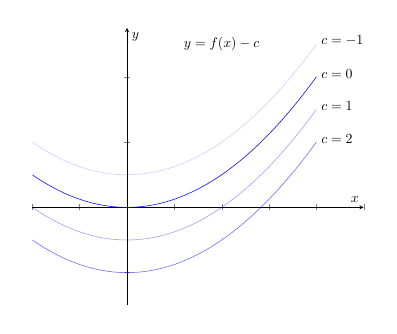
\begin{tikzpicture}[scale=0.5]
\begin{axis}[
 axis lines=middle,
 ticklabel style={fill=white},
xmax=2.5,
 ymin=-3,  ymax=5.5,
 xlabel=$x$,ylabel=$y$,
 samples=100,
 smooth,
xticklabels=\empty, yticklabels=\empty,
 width=10cm]

\addplot[blue,  domain=-1:2, opacity=0.2] {(x)^2+1};
\addplot[blue,  domain=-1:2] {x^2};
\addplot[blue, domain=-1:2, opacity=0.4] {(x)^2-1};
\addplot[blue, domain=-1:2, opacity=0.6] {(x)^2-2};
%\addplot[blue] {(x-2)^2};
\node[] at (axis cs:1,5) {$y=f(x)-c$};
\node[right] at (axis cs:2,2^2+0.1) {$c=0$};
\node[right] at (axis cs:2,2^2+1+0.1) {$c=-1$};
\node[right] at (axis cs:2,2^2-1+0.1) {$c=1$};
\node[right] at (axis cs:2,2^2-2+0.1) {$c=2$};
\end{axis}
\end{tikzpicture}